
\section{Introduction}
%\cd{TODO - fix line "When the background is subtracted, all variation in the as well as the standard deviation is reduced to flat line, with little noise."}
Cloud providers offer FPGAs as a service. The versatility of FPGAs makes them efficient compute engines for neural networks~\cite{fowers2018configurable}, genome sequencing~\cite{chen2016spark}, secure database transactions~\cite{arasu2015transaction}, networking~\cite{putnam2014reconfigurable}, and homomorphic encryption~\cite{poppelmann2015accelerating}. These applications have strict requirements for data confidentiality and computational integrity. 



%To satisfy the security requirements,
FPGA cloud providers use strict time-sharing schemes where a user rents the entire FPGA. This can leave the FPGA under-utilized. FPGA virtualization maximizes utilization by supporting multiple concurrent users~\cite{zha2020virtualizing}. It can reduce costs and increase efficiency, making it an attractive option for cloud service providers.

Unfortunately, FPGA virtualization introduces a side channel observable by an attacker implementing a \sensor within their programmable logic. \Sensors measure minute voltage changes in the power distribution network that expose details about co-tenant computations. \Sensors are used as a covert channel~\cite{zhao2018fpga, schellenberg2018remote} or a side channel to extract cryptographic keys of co-located encryption cores~\cite{zhao2018fpga, schellenberg2018remote}. 

\begin{figure}[t!]
\centering
\vspace{-5px}
%
\includegraphics[scale=.5]{img/optimization_intro_revised.pdf}
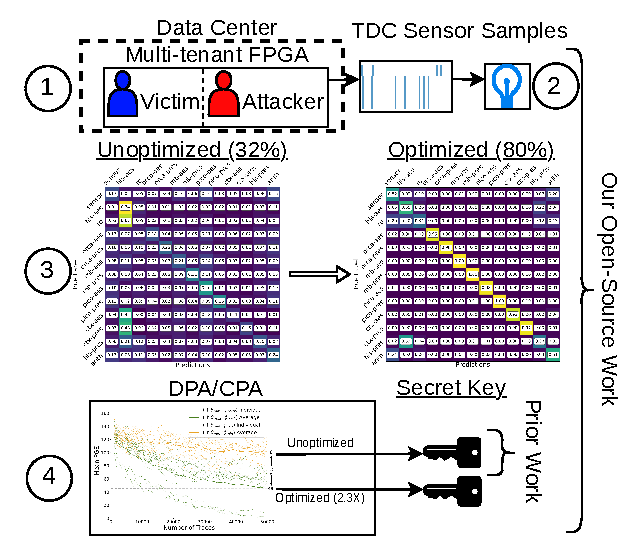
\includegraphics[scale=.85]{img/ASPLOS_Big_Picture.pdf}
\vspace{-10px}
\caption{\textcircled{\raisebox{-.8pt} {1}} An attacker spatiotemporally locates with a victim. % to extract information about the victim's computation. 
\textcircled{\raisebox{-.8pt} {2}} The attacker instantiates our \name TDC. % that measures the shared power distribution network. 
\textcircled{\raisebox{-.8pt} {3}} Our dynamic tuning techniques improve the ability to classify victim co-tenant computation by 2.5$\times$. \textcircled{\raisebox{-.8pt} {4}} After recognizing a cryptographic core, dynamic tuning increases the effectiveness of correlation power analysis by 2.2$\times$.
%\dr{Where did spatiotemporally come from? It would be cool to sneak 2.5x and 2.2x into the figure.} \cd{I do not know who added spatiotemporally, but it makes sense to me. Figure updated.} \rk{Guilty! I also learned that spatiotemporal and temporospatial are both words that seem to be equivalent? Happy to be educated on the difference. We should probably settle on one or the other if we are using both.}
%Stages 1-4 provide a pipeline for optimizing side channel sensor readings, correctly determining co-located computation, and performing a key recovery attack. }
%\cd{TODO - squish if possible. Open source hyphenated?
}
\label{fig:intro_fig}
\vspace{-10px}
\end{figure}

%This paper examines the design, analysis, and optimization of 
\emph{Time-to-Digital Converters (TDCs)} are a common \sensor that measure the propagation delay through a linear array of logic elements, which is a function of the \emph{power distribution network (PDN)} voltage. A slower propagation indicates that the PDN is stressed by some computation. These voltage fluctuations over time can be measured with consecutive TDC output captures.



Figure~\ref{fig:intro_fig} shows our open-source pipeline. In Stage \textcircled{\raisebox{-.8pt} {1}}, an attacker co-locates temporospatially with a victim user. %An FPGA bitstream with multiple logically and physically isolated designs is used to emulate this multi-tenant structure. 
The attacker measures the shared power distribution network in Stage \textcircled{\raisebox{-.8pt} {2}}. Our open-source \textit{\name TDC} allows the attacker to dynamically tune its sensing parameters, including transition polarity, sample window, frequency, and phase. Previously proposed TDC sensors are statically tuned in one or more of these parameters, which requires detailed knowledge of the computational environment and target computation. Utilizing these techniques in Stage \textcircled{\raisebox{-.8pt} {3}}, we demonstrate that a well-tuned sensor can improve classification accuracy by 2.5$\times$ over a statically-tuned sensor that incorrectly characterizes its environment or target computation. After successfully classifying an AES computation, we demonstrate in Stage \textcircled{\raisebox{-.8pt} {4}} that proper sensor calibrations increase the ability to correctly rank subkey values by 2$\times$ in a Correlation Power Analysis (CPA) attack.


%A fundamental contribution of this work is to optimize these measurements to enhance the information about the attacker's computation that is encoded in the TDC sensor readings. Optimizing the TDC sensor allows the attacker to more effectively extract information about the victim computation, e.g., performing a key extraction attack. 

%To emulate a true multi-tenant model of \textcircled{\raisebox{-.9pt} {1}}, a standard FPGA bitstream with multiple logically and physically isolates designs is used. Stage \textcircled{\raisebox{-.9pt} {2}} utilizes three optimization techniques afforded to the attacker by our open-source \textit{\name TDC} which is novel in its ability to dynamically tune its sensing parameters including transition polarity, sample window, and phase. Utilizing these techniques in Stage \textcircled{\raisebox{-.9pt} {3}}, we demonstrate that a well-tuned sensor can improve classification accuracy by 2.5$\times$. The data and classification network have also been open sourced. After successfully identifying an AES computation with our classification process, we demonstrate in Stage \textcircled{\raisebox{-.9pt} {4}} that proper sensor calibrations increases the ability to correctly rank subkey values  by 2$\times$ using a Correlation Power Analysis (CPA) attack.

%We examine how these features improve the sensor's ability to capture information about a co-tenant and improve cross-board generalization. Finally, we examine how the tuning phase relationship between the \name TDC and the co-tenant clock influences the ability to capture side-channel leakage. 

%These tactics are employed in a 13-way classification task where an attacker is attempting to learn about the architecture and algorithm running in a multi-tenant environment in order to perform a side-channel attack. 

%Our experiments demonstrate that transition polarity, metric selection, phase and duration tuning, and background subtraction, are important factors in maximizing channel information and a well tuned sensor can improve classification accuracy by 2.5$\times$. After successfully identifying an AES computation with our classification network, we demonstrate that proper sensor calibrations increases the frequency with which all correct subkey values are ranked as most likely by 2$\times$ in a Correlation Power Analysis attack.



The contributions of this work are:
\begin{itemize}
    \item An Open-Source \name TDC sensor for performing side-channel attacks on FPGAs
    \item A study of our sensor implementation on both Intel and Xilinx platforms.
    \item A study of three metrics for measuring the propagation distance of rising and falling transitions
    \item A technique for maximizing channel information by adjusting capture window duration
    \item A method for tuning to the unknown phase of a co-tenant computation and isolating it from the environment
    \item A study characterizing the impact of these parameters on a 13-application, cross-board classification problem
    \item An application of our tuning methods to a multi-tenant Correlation Power Analysis attack
\end{itemize}

To the best of our knowledge, this is the first work to demonstrate a tuning feature to minimize the phase difference between a \sensor and a victim computation. We describe this novelty in great detail in Section \ref{target_clock_tuning} and contrast it to prior work in Section \ref{related}. As an improvement to our prior work, we demonstrate the portability of our \sensor design to Intel FPGA architectures. To maintain the resolution of our sensor on Intel FPGA systems, we present a novel PLL configuration preprocessing algorithm that provides fine-grained phase stepping capabilities to FPGA systems with low resolution PLL phase increment specifications.

The paper is organized as follows:
Section~\ref{threat_model} presents the threat model.
Section~\ref{sensor_structure} describes our \name TDC and its tuning abilities on Xilinx and Intel architectures.
%Section~\ref{results} discusses the experimental results which show how tuning enables the \name TDC to extract more information about the co-tenant computations. 
Section~\ref{results} experimentally verifies the tuning optimizations presented in the previous section and shows how this can be leveraged to perform our classification attack as well as a Correlation Power Analysis. We conclude in Section~\ref{conclusion}. 